%~~~~~~~~~~~~~~~~~~~~~~~~~~~~~~~~~~%
%   PIERO CAMPALANI                %
%   Curriculum-vitae               %
%~~~~~~~~~~~~~~~~~~~~~~~~~~~~~~~~~~%

% workarond for bibentry/hyperref compatibility issues
% http://www.tug.org/applications/hyperref/ftp/README
\makeatletter
\let\saved@bibitem\@bibitem
\makeatother
% --------- %

\pdfminorversion=4
\documentclass[10pt]{article}
\usepackage[margin=3cm]{geometry}
\usepackage{marvosym}		% mobile phone symbol
\usepackage{textcomp}		% born symbol
\usepackage{fixltx2e}		% text subscript
\usepackage{titling}		% vspace title/author
\posttitle{\par\end{center}}
\usepackage{fancybox, graphicx}
\usepackage{longtable}		% tables across pages
\setlength{\LTpre}{0pt}
\setlength{\LTpost}{0pt}
\usepackage{bibentry}
\usepackage{hyperref}		% hyperlinks
\graphicspath{{./pics/}{/usr/share/doc/texlive-doc/latex/minitoc/}}	% countries flags
\DeclareGraphicsExtensions{.pdf,.png,.jpg}
\DeclareMathAlphabet{\mathpzc}{OT1}{pzc}{m}{it}	% mathzpc style

% New definitions
% For RGB hexs, see: http://www.html.am/html-codes/color/color-code-chart.cfm
\usepackage[table,usenames,dvipsnames]{xcolor}
\definecolor{grey}{gray}{0.2}
\definecolor{medgrey}{gray}{0.5}
\definecolor{lightgray}{gray}{0.8}
\definecolor{verylightgray}{gray}{0.95}
\definecolor{palegoldenrot}{HTML}{EEE8AA}
\definecolor{lightgoldenrodyellow}{HTML}{FAFAD2}
\definecolor{lightslategrey}{HTML}{778899}
\newcolumntype{L}{>{\raggedleft}p{0.14\textwidth}}
\newcolumntype{R}{p{0.8\textwidth}}
\newcommand\VRule{\color{lightgray}\vrule width 0.7pt}

\usepackage{colortbl}

% hyperref defaults
% http://stackoverflow.com/questions/544907/remove-boxes-from-hyperlinked-toc-in-latex
\hypersetup{%
    pdfborder = {0 0 0}
}


% TITLE ~~~~~~~~~~~~~~~~~~~~~~~~~~~~~~~~~~~~~~~~~~~~~~~~~~
\title{\bfseries\Huge Piero Campalani}
%\author{\emph{curriculum vitae}\thanks{Last update: \today.}} -- puts a line in the second page..
\author{\emph{curriculum vitae}\textsuperscript{*}}
\date{}

\pagenumbering{roman}

\begin{document}
\maketitle
\let\thefootnote\relax\footnote{\textsuperscript{*}Last update: \today.}

% PERSONAL INFO ~~~~~~~~~~~~~~~~~~~~~~~~~~~~~~~~~~~~~~~~~~
\vspace{-.5cm}
\begin{minipage}[ht]{0.2\textwidth}
\raggedright
  \shadowbox{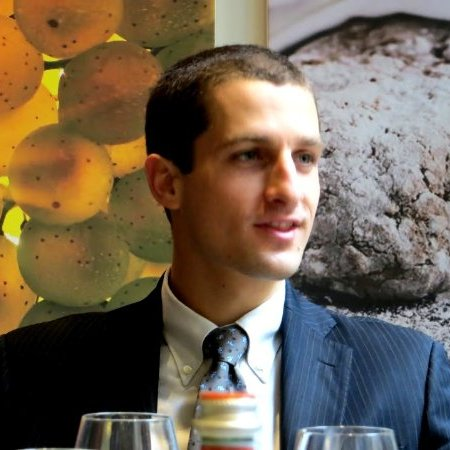
\includegraphics[width=2.2cm]{avatar}}
\end{minipage}
\begin{minipage}[ht]{0.33\textwidth}
  \begin{flushleft}
  \begin{tabular}{ c l }
    \textborn & 1985 November 1\textsuperscript{st}\\
              & Portomaggiore (FE), IT\\
    \Mobilefone & 
\includegraphics[width=3mm]{italy-f}   $\mathpzc{{\scriptstyle +}39\,333\,412\,83\,17}$\\
%                & 
\includegraphics[width=3mm]{germany-f} $\mathpzc{{\scriptstyle +}49\,152\,101\,59\,244}$
                & 
\includegraphics[width=3mm]{spain-f} $\mathpzc{{\scriptstyle +}34\,611\,209\,861}$
  \end{tabular}
  \end{flushleft}
\end{minipage}
\begin{minipage}[ht]{0.33\textwidth}
  \begin{flushright}
  \begin{tabular}{ c l }
    \Letter & Via della Resistenza n.18\\
           & 44121 Ferrara, IT\\
    {\small \MVAt} & \href{mailto:piero.campa@gmail.com}{\texttt{piero.campa@gmail.com}}\\[3pt]
    
\includegraphics[width=3.5mm]{earth-logo} &
                    \href{https://www.ohloh.net/accounts/pierocampa}{
\includegraphics[width=4mm]{ohloh-logo}}
                    \href{https://www.researchgate.net/profile/Piero_Campalani/}{
\includegraphics[width=4mm]{researchgate-logo}}
                    \href{https://www.linkedin.com/pub/piero-campalani/19/4a6/b13}{
\includegraphics[width=4mm]{linkedin-logo}}
                    \href{https://careers.stackoverflow.com/users/info/189094}{\includegraphics[width=4mm]{{careers2.0-logo}.pdf}}
  \end{tabular}
  \end{flushright}
\end{minipage}
\vspace{.5cm}

% SUMMARY ~~~~~~~~~~~~~~~~~~~~~~~~~~~~~~~~~~~~~~~~~~~~~~~~
\section*{In Short}
\small
Self-committed and motivated researcher, I love tackling new challenges and implementing.
On my way through \textbf{\mbox{\emph{geo}-informatics}}, I feel more comfortable inside \mbox{open-source} collaborative environments.
I believe in the importance of open discussions and peopleware, in preemptive analysis and design (and in code comments).

After graduating as TLC \emph{engineer} in the University of Ferrara, I gained experience as spatial analyst for air quality applications
during my PhD, developing geostatistical multivariate models for particles exposure mapping, with satellite imagery.

During my \emph{postdoctoral fellowship} in the Jacobs University in Bremen, I am (currently) working on the design
and implementation of OGC geo-image web services (WCS\slash WCPS) for visualization and server-side processing
of Big spatio-temporal gridded datasets via the \mbox{open-source} \texttt{rasdaman} project.
~\\ ~\\
In the recent years I have been working continuously in highly \textbf{international environments},
developing side by side with my team members, tutoring students and providing continuous support to
the \mbox{\textbf{open-source}} community willing to use our software.

I have been presenting the proceedings of my research at several international
scientific conferences and symposiums.
I am able to summarize the key aspects of a work and present it in a proper manner to others,
leveraging the level of details to the different contexts: from the short presentation to domain outsiders
up to more technical tutorials for full dedicated workshops.

Technically, I am a Linux user since years; I am fond of many programming languages
(e.g.~Java, Bash, R, or C\slash C++); I have been designing and implementing active
PostgreSQL databases; I am a \textsl{git}-enthusiast and I can easily deal with distributed and versioned development.
Finally, when it comes to exhibit the results I like to be assisted by Inkscape, Gimp and \LaTeX{}.


% OCCUPATIONAL FIELD ~~~~~~~~~~~~~~~~~~~~~~~~~~~~~~~~~~~~~
\section*{Desired Occupational Fields}
{\normalsize Spatial Analysis and Modelling $\cdots$ Remote Sensing $\cdots$ Computer Science $\cdots$ Telecommunications.}

\pagebreak
% PROFESSIONAL EXPERIENCE ~~~~~~~~~~~~~~~~~~~~~~~~~~~~~~~~
\section*{Professional Experience}
\begin{longtable}{L!{\VRule}R}
\rowcolor{SpringGreen}
2015--\emph{now}& \textbf{Development Engineer} at Ebotlution Systems S.L., Barcelona, Spain.\\
              & \footnotesize\textit{Engineering innovative solutions for optimized mine clearance in the field of 
               Humanitarian Demining: automated mine/UXO detection via droids, real-time telemetry monitoring, multi-actor 
               multi-point network protocol definition, advanced GIS user interface with decision-support systems}
               --- the initiative is a recognized R\&D project.\\[5pt]
\rowcolor{verylightgray}
2013--2014& \textbf{PostDoc} in the Large-Scale Scientific Information Systems (LSIS) Research Group at Jacobs University, Bremen, Germany.\\
             & \footnotesize\textit{Design and development for Web-based access and analysis of time series of regularly and irregularly
               gridded geo-images through the \textnormal{\texttt{rasdaman}} Array DBMS and its Java servlet. Active role in
               the OGC ``Temporal Ad-Hoc'' Working Group for the definition of spatio-temporal Coordinate Reference Systems for coverages}
               --- research grant from the EU~FP7 ``EarthServer'' project.\\[5pt]
\rowcolor{verylightgray}
2012--2013   & \textbf{PhD guest} in the Large-Scale Scientific Information Systems (LSIS) Research Group at Jacobs University, Bremen, Germany.\\
             & \footnotesize\textit{12 months of research and development activity on the \textnormal{\texttt{rasdaman}} Array DBMS and its Java Web
               interface for online access of raster geo-images. International research team, collaborative FOSS software
               development, OGC services (WCS, WCPS, WMS) implementation and design} --- research grant from the EU~FP7 ``EarthServer'' project.\\[5pt]
%$\Downarrow$ &\\[5pt]
\rowcolor{verylightgray}
2010--2012   & \textbf{PhD internship} at MEEO Srl, Ferrara, Italy.\\
             & \footnotesize\textit{23 months of research on the evaluation of spaceborne MODIS maps of Aerosol Optical Thickness
               for the gap-filling of surface PM\textsubscript{10} exposures. Development of multivariate kriging models with \textnormal{\texttt{R}},
               satellite maps validation through uplooking sunphotometers and implementation of a Web GIS
               interface for the visualization of ground-based,
               remote sensing, and model-based air quality datasets} --- research grant from the european
               ``SENSing, mOdeling and distRibution of EnviRonmental data (SENSORER)'' regional development project.
\end{longtable}

% EDUCATION ~~~~~~~~~~~~~~~~~~~~~~~~~~~~~~~~~~~~~~~~~~~~~~
\vspace{.5cm}
\section*{Education}
\begin{longtable}[t]{L!{\VRule}R}
\rowcolor{SkyBlue}
2010--2012& \textbf{PhD} in \textsl{Engineering Sciences} at Universit\`a degli Studi di Ferrara, Italy.\\[-2pt]
          & \footnotesize\emph{Thesis title:} Geostatistical modelling of PM$_{10}$ mass concentrations with satellite imagery from MODIS sensor\\[-2pt]
          & \footnotesize\emph{Final degree mark:} Ottimo\\[-2pt]
          & \footnotesize\emph{PhD cycle:} XXV\\[-2pt]
          & \footnotesize\emph{Duration:} 3 years\\[7pt]
\rowcolor{verylightgray}
      2009& Professional habilitation (\textbf{Esame di Stato}) as \textsl{Information Engineer} at Universit\`a di Bologna, Italy.\\[-2pt]
          & \footnotesize\emph{Category:} Nuovo Ordinamento, section A\\[-2pt]
          & \footnotesize\emph{Final examination mark:} 211\slash 240\\[7pt]
\rowcolor{verylightgray}
2007--2009& \textbf{MSc} in \textsl{Electronic and Telecommunications Engineering} at Universit\`a degli Studi di Ferrara, Italy.\\[-2pt]
          & \footnotesize\emph{Thesis title:} Architectures and Perfomance for Network Coding\\[-2pt]
          & \footnotesize\emph{Final degree mark:} 110\slash 110 cum laude\\[-2pt]
          & \footnotesize\emph{Duration:} 2 years\\[7pt]
\rowcolor{verylightgray}
2004--2007& \textbf{BSc} in \textsl{Electronic and Telecommunications Engineering} at Universit\`a degli Studi di Ferrara, Italy.\\[-2pt]
          & \footnotesize\emph{Thesis title:} Robust Hash for Audio Identification\\[-2pt]
          & \footnotesize\emph{Final degree mark:} 109\slash 110 \\[-2pt]
          & \footnotesize\emph{Duration:} 3 years \\[7pt]
\rowcolor{verylightgray}
1999--2004&Scientific secondary school diploma at Liceo Scientifico A. Roiti, Ferrara, Italy.\\[-2pt]
          & \footnotesize\emph{School-leaving examination mark:} 88\slash 100
\end{longtable}


% TRAINING COURSES ~~~~~~~~~~~~~~~~~~~~~~~~~~~~~~~~~~~~~~~
\pagebreak
\vspace{.5cm}
\section*{Training Courses}
\begin{longtable}{L!{\VRule}R}
\rowcolor{palegoldenrot}
2017 & \textbf{Geo-computation using free and open source software} Summer School at the University of Basilicata in Matera, Italy.\\[-2pt]
     & \footnotesize\emph{Description:} R, Grass, Python, Gdal/Ogr library and the Linux operating system.\\[-2pt]
     & \footnotesize\emph{Duration:} 5 days\\[7pt]
\rowcolor{lightgoldenrodyellow}
2014 & \textbf{Monitoring of the Earth System} Summer School at ESA\slash ESRIN, Italy.\\[-2pt]
     & \footnotesize\emph{Description:} \textsc{Global Observing Systems}: Capabilities and applications of Earth Observation,
physics of remote sensing measurement, concept of integrated Observing Systems of Systems.
\textsc{Earth System Modelling}: Basics of ocean, atmosphere, land and ice modelling, Numerical Weather Prediction, ensemble forecasting.
\textsc{Data Assimilation}: Theory of data assimilation techniques (e.g. optimal interpolation, variational methods,
Kalman filter, ensemble filtering) and applications (e.g. re-analysis, inverse modelling, state estimation,
control theory, design of optimal observing system, targeting observations).
\textsc{Global Change}: Observation of global change from space, use of Earth System model to understand, forecast and manage environmental issues.\\[-2pt]
     & \footnotesize\emph{Duration:} 10 days\\[7pt]
\rowcolor{palegoldenrot}
2013 & \textbf{Basic Aerosol Science} Summer School at the Faculty of Physics of the University of Vienna, Austria.\\[-2pt]
     & \footnotesize\emph{Description:} Introduction into aerosol mechanics; interaction of light with particles;
nucleation and condensation phenomena; electrical aerosol measurement; diffusion and particle filtration;
fundamental chemistry of the aerosol system; chemical on line measurement; modern spectroscopy as a tool for aerosol characterization;
interaction of aerosol particle with the lung: deposition, clearance and retention; primary bio particles;
optical particle measurement; visibility and atmospheric optics; inertial separators;
remote sensing of atmospheric aerosols; monitoring and data anlysis.\\[-2pt]
     & \footnotesize\emph{Duration:} 10 days\\[7pt]
\rowcolor{lightgoldenrodyellow}
2012 & \textbf{GEOSTAT} Summer School at the Institute for Geoinformatics of the University of M\"unster, Germany.\\[-2pt]
     & \footnotesize\emph{Description:} Spatial and spatio-temporal data analysis in \texttt{R}; \texttt{R} as a GIS; visualization of spatio-temporal data from \texttt{R} to Google Earth, GRASS GIS and SAGA GIS tutorials; spatial aggregation and change of support in geostatistics; spatio-temporal geostatistics.\\[-2pt]
     & \footnotesize\emph{Duration:} 6 days\\[7pt]
\rowcolor{palegoldenrot}
2011 & \textbf{Analysing Spatial Data} intensive PhD course by Prof.~Roger Bivand at the Norwegian School of Economics (NHH), Bergen, Norway.\\[-2pt]
     & \footnotesize\emph{Description:} Introduction to \texttt{R}; representing spatial data in conceptual and practical terms;
       non-spatial visualisation and analysis of spatial data; the analysis of point patterns; interpolation and geostatistics;
       areal data and spatial econometrics; project preparation, supervision, and presentation. \\[-2pt]
     & \footnotesize\emph{Duration:} 8 days\\[7pt]
\end{longtable}

\pagebreak
% WORKSHOPS  ~~~~~~~~~~~~~~~~~~~~~~~~~~~~~~~~~~~~~~~
\definecolor{MidnightBlue}{RGB}{25,25,112} % http://cloford.com/resources/colours/500col.htm
\vspace{.5cm}
\section*{\underline{T}alks\slash \underline{W}orkshops}
\begin{longtable}{L!{\VRule}R}
2014/07 & \textcolor{OrangeRed}{\scriptsize{[W]}}
          \textcolor{MidnightBlue}{\textit{``Spatio-Temporal Big Data --- the} rasdaman \textit{approach''}}\\[-2pt]
        & \textsc{OSGeo's European Conference on Free and Open Source Software for Geospatial} (Bremen, DE).\\[2pt]
2014/06 & \textcolor{Orange}{\scriptsize{[T--KEYNOTE]}}\textcolor{MidnightBlue}{\textit{``Server-side Maps Processing
          for the Air Quality with the WCPS Standard''}}\\[-2pt]
        & \textsc{International Workshop on Air Quality in Asia} (Hanoi, VN).\\[2pt]
        & \textcolor{OrangeRed}{\scriptsize{[W]}}
          \textcolor{MidnightBlue}{\textit{``Spatio-Temporal Big Data --- the} rasdaman \textit{approach''}}\\[-2pt]
        & \textsc{Open Source Geospatial Research and Education Symposium} (Espoo, FI).\\[2pt]
2014/04 & \textcolor{Orange}{\scriptsize{[T]}}
          \textcolor{MidnightBlue}{\textit{``EarthServer: Agile Analytics on Big Earth Data''}}\\[-2pt]
        & \textsc{Ecosystem approach to marine data workshop} (Athens, GR).\\[2pt]
2014/03 & \textcolor{Orange}{\scriptsize{[T]}}
          \textcolor{MidnightBlue}{\textit{``A Proposal for Temporal and Index CRSs for OGC-NA''}}\\[2pt]
        & \textsc{OGC Technical Committee Meeting} (Crystal City, VA, USA).\\[2pt]
2013/06 & Attendance to \textsc{Big Data From Space} (ESA\slash ESRIN, IT)\\[2pt]
2013/03 & \textcolor{Orange}{\scriptsize{[T]}}
          \textcolor{MidnightBlue}{\textit{``Multi-Dimensional Space \& Time Support by Coordinate Reference Systems''}}\\[-2pt]
        & \textsc{OGC Technical Committee Meeting} (Abu Dhabi, UAE).\\[-2pt]
\end{longtable}

% LANGUAGES ~~~~~~~~~~~~~~~~~~~~~~~~~~~~~~~~~~~~~~~~~~~~~~
\vspace{.5cm}
\section*{Languages}
\begin{longtable}{L!{\VRule}R}
Italian & Mother tongue\\[3pt]
English & Upper-intermediate\\[-2pt]&\scriptsize\emph{12\slash 2010 Cambridge FCE certification (B2 CEFR level) -- Grade A}\\[3pt]
Spanish & Upper-intermediate\\[-2pt]&\scriptsize\emph{05\slash 2013 DELE certification (B2 CEFR level)}\\[3pt]
German  & Intermediate
\end{longtable}

% MAIN SKILLS ~~~~~~~~~~~~~~~~~~~~~~~~~~~~~~~~~~~~~~~~~~~~
\vspace{.5cm}
\section*{Skills}
\begin{longtable}{L!{\VRule}R}
\emph{Domains} & Spatial analysis and geostatistics\\[-2pt]
               & Autonomous navigation systems\\[-2pt]
               & OGC Web services for coverages (WCS\slash WCPS)\\[5pt]
\emph{Technical} & GIS applications\\[-2pt]
                 & DBMS management\\[-2pt]
                 & Collaborative software development\\[-2pt]
                 & Radio communications\\[-2pt]
                 & Kalmann filters\\[5pt]
\emph{Programming} & Java, C{}\verb!++!, R, bash, psql, PL\slash pgSQL, C, C\#, MATLAB, Python.\\[5pt]
\emph{Software} & Eclipse\slash NetBeans IDEs, git, PostgreSQL, GDAL, OpenLayers, MapProxy, MapServer, PostGIS, \LaTeX.\\[5pt]
\emph{OS}       & Linux (Ubuntu), Windows.
\end{longtable}

\pagebreak
% BIBLIOGRAPHY ~~~~~~~~~~~~~~~~~~~~~~~~~~~~~~~~~~~~~~~~~~~
\vspace{.5cm}
\bibliographystyle{abbrv}
%\nobibliography{mybibliography}
% hyperref-bibentry compatibility workaround
\begingroup
  \makeatletter
  \let\@bibitem\saved@bibitem
  \nobibliography{mybibliography}
\endgroup
% -------- %
\section*{Publications}
\begin{longtable}{L!{\VRule}R}
\textbf{2015} & \textcolor{lightslategrey}{\bibentry{es2015overarching}.}\\[10pt]
\textbf{2014} & \bibentry{campalani2014atmosphere}.\\[5pt]
              & \bibentry{yu2014gis}.\\[5pt]
              & \textcolor{lightslategrey}{\bibentry{yu2014point}.}\\[10pt]
\textbf{2013} & \bibentry{campalani2013integration}.\\[5pt]
              & \bibentry{campalani2013referenceable}.\\[5pt]
              & \bibentry{campalani2013spatiotemporal}.\\[5pt]
              & \textcolor{lightslategrey}{\bibentry{oosthoek2013towards}.}\\[5pt]
              & \textcolor{lightslategrey}{\bibentry{oosthoek2013innovative}.}\\[10pt]
\textbf{2012} & \bibentry{baumann2012finding}.\\[5pt]
              & \bibentry{campalani2012prediction}.\\[5pt]
              & \textcolor{lightslategrey}{\bibentry{nguyen2012aerosol}.}\\[10pt]
\textbf{2011} & \bibentry{campalani2011prediction}.\\[5pt]
              & \bibentry{campalani2011validation}.\\[5pt]
              & \textcolor{lightslategrey}{\bibentry{natali2011mea-pm}.}\\[10pt]
\textbf{2010} & \textcolor{lightslategrey}{\bibentry{nguyen2010aerosol}.}\\[5pt]
              & \bibentry{sensorer0154}.\\[5pt]
              & \bibentry{sensorer0153}.\\[5pt]
              & \bibentry{sensorer0152}.\\
\end{longtable}

% signature
\vspace{1.5cm}
\begin{figure}[h]
  \raggedleft
  
\includegraphics[width=40mm]{firma}
\end{figure}

\end{document}
